\documentclass[letterpaper,12pt]{article}

\usepackage[english,spanish]{babel}
\usepackage[utf8]{inputenc}
\usepackage{graphicx} % Add graphics capabilities
\usepackage{booktabs} % ``Proper'' table layout
\usepackage{amsmath}  % Better maths support
\usepackage{amssymb} 
\usepackage{amsthm}
\usepackage[colorlinks=true,linkcolor=red]{hyperref} % Hyperlink capabilities
\usepackage{memhfixc} 
\usepackage{makeidx} 
% This package is required to resolve incompatibilities with the memoir class 
% & the hyperref package   
\usepackage[font=scriptsize]{caption}
\usepackage[font=scriptsize]{subcaption}  
\usepackage{tikz}
\usepackage{bbm}
\usepackage{bm}
\usepackage{footnote}
\usetikzlibrary{arrows}
\usetikzlibrary{automata}
\theoremstyle{definition} \newtheorem{Def}{Definición}[section]
\theoremstyle{definition} \newtheorem{Teo}{Teorema}[section]
\theoremstyle{definition} \newtheorem{Pro}{Proposición}
\theoremstyle{definition} \newtheorem{Lema}{Lema}[section]
\theoremstyle{definition} \newtheorem{Cor}{Corolario}[section]
\author{Alejandro Nieto Ramos}
\title{Modelado y simulación de datos de crecimiento tumoral usando modelos de efectos mixtos}
\date{2 de agosto de 2016}
\begin{document}

\maketitle

\section{Introducción}

En el artículo \emph{A Tumor Growth Model for Low-Grade Glioma treated with Chemotherapy or Radiotherapy} de Benjamin Ribba et al, se presenta un modelo de la inhibición del crecimiento tumoral de gliomas difusos de grado bajo (LGG) -un tipo de tumor cerebral- en adultos. Este modelo es capaz de describir la evolución del tamaño de tumores en los pacientes tratados con quimioterapia y radioterapia. El objetivo de este documento es replicar los resultados del artículo obtenidos con Monolix y simplificar el modelo para ver observar qué sucede.

En el artículo, se utilizaron datos de la media del diámetro longitudinal del tumor (MTD)\footnote{Calculada de acuerdo a $MTD=\sqrt{2D}$, donde $V=\frac{1}{2} D_1 D_2 D_3$ es el volumen aproximado del tumor y $D_i, \, i=1,2,3,$ son los tres diámetros perpendiculares más grandes del tumor.} en 21 pacientes tratados por primera vez, a quienes se les administró  procarbazina, nitrosourea (1-(2-Chloroethyl)-3-cyclohexylurea) y vincristina (PCV). Se formuló un modelo a base de ecuaciones diferenciales en el cual se incorporaron tanto parámetros específicos del tumor y como relacionados con el tratamiento, que reflejan la respuesta del tejido tumoral proliferativo y latente. El modelo se aplicó después a datos del tamaño longitudinal de tumores en 24 pacientes de primera vez a quienes se les administró temozolamida (TMZ) y a 25 pacientes de primera vez también tratados con radioterapia. 

De acuerdo a los autores, el modelo intenta capturar la cinética del crecimiento de los LGG en pacientes tratados con quimioterapia o radioterapia y finalmente como herramienta que permita predecir la eficacia del tratamiento de los LGG así como mejorar el esquema de tratamiento. Se señala que en un estudio hecho anteriormente por ellos mismos, se demostró que una vez terminado el tratamiento con PVC, el volumen de los LGG disminuía a pesar de no recibir más quimioterapia; que una posible causa de este efecto pudiera ser la acción retardada de la quimioterapia en las células latentes del tumor, y que la hipótesis es consistente con el mecanismo de acción del ciclo celular de los agentes alquilos usados en el tratamiento con PVC. Por lo tanto, formularon un modelo de la inhibición del crecimiento del tumor que tomara en cuenta células del tumor ploliferativas y latentes porque responden de manera diferente al tratamiento. 

\section{La técnica de modelado}

El modelo de tumor pertenece a a categoría de los modelos de efectos mixtos. Mediante esta técnica, todos los datos individuales se analizan simultáneamente para dar información de la evolución de cada tumor individual. Por otro lado, el proceso de modelado consta de dos etapas. En el primero, se minimiza una función de verosimilitud para estimar los valores medios de los parámetros del modelo así como la variabilidad individual de los mismos en la población. A los estimadores resultantes se les conoce como parámetros de la población. En el segundo paso, se usa la información de los parámetros de la población para estimar el mejor los mejores parámetros del modelo para cada individuo con base en su propio conjunto de datos. A estos parámetros se les llama parámetros individuales. Monolix está basado en la aproximación estocástica del algoritmo de esperanza maximizacion y es el software que se usó para estimar tanto los parámetros de la población como los individuales.
\section{La estrategia}

Existen dos razones por las cuales los autores escogieron la serie de datos correspondientes al tratamiento PCV y no las otras dos. La primera que mencionan es que para ellos era esencial que su modelo pudiera describir la disminución de la MTD que ocurre después de terminado el tratamiento, pensando que se debe al resultado de las diferentes respuestas que tienen los dos tipos de células. En particular, señalan esta disminución es particularmente clara en el caso del tratamiento con PVC. Por otro lado, el conjunto de datos en este último caso fue el más completo, con un periodo de observación más largo y con el mayor número de observaciones por paciente antes y después del tratamiento. 

\section{El modelo}
El modelo usado por por los autores se muestra en la figura (\ref{modelo}). El tumor está formado de células proliferativas (P) y tejido latente no proliferativo  (Q), expresado en milímetros. La transición del tejido proliferativo a latente está dictada por la tasa constante $k_{PQ}$. El tratamiento elimina directamente células proliferativas al inducir daño letal en el ADN mientras las células se desarrollan mediante el ciclo celular. Las células latentes también se ven afectadas por el tratamiento y se convierten en células latentes dañadas $(Q_p)$. Estas células, cuando nuevamente forman parte del ciclo celular, pueden o bien reparar su ADN y convertirse nuevamente en proliferativas (transición de $Q_p$ a $P$), o pueden morir por daños irreparables. De acuerdo a los autores, esta hipótesis es consistente con el mecanismo de acción de los agentes alquilantes CCNU y procarbazina, a los cuales se les considera medicamentos no específicos del ciclo celular que inducen daños en el ADN, tanto en el tejido proliferativo como en el latente. 

\begin{figure}[h]
	\centering
	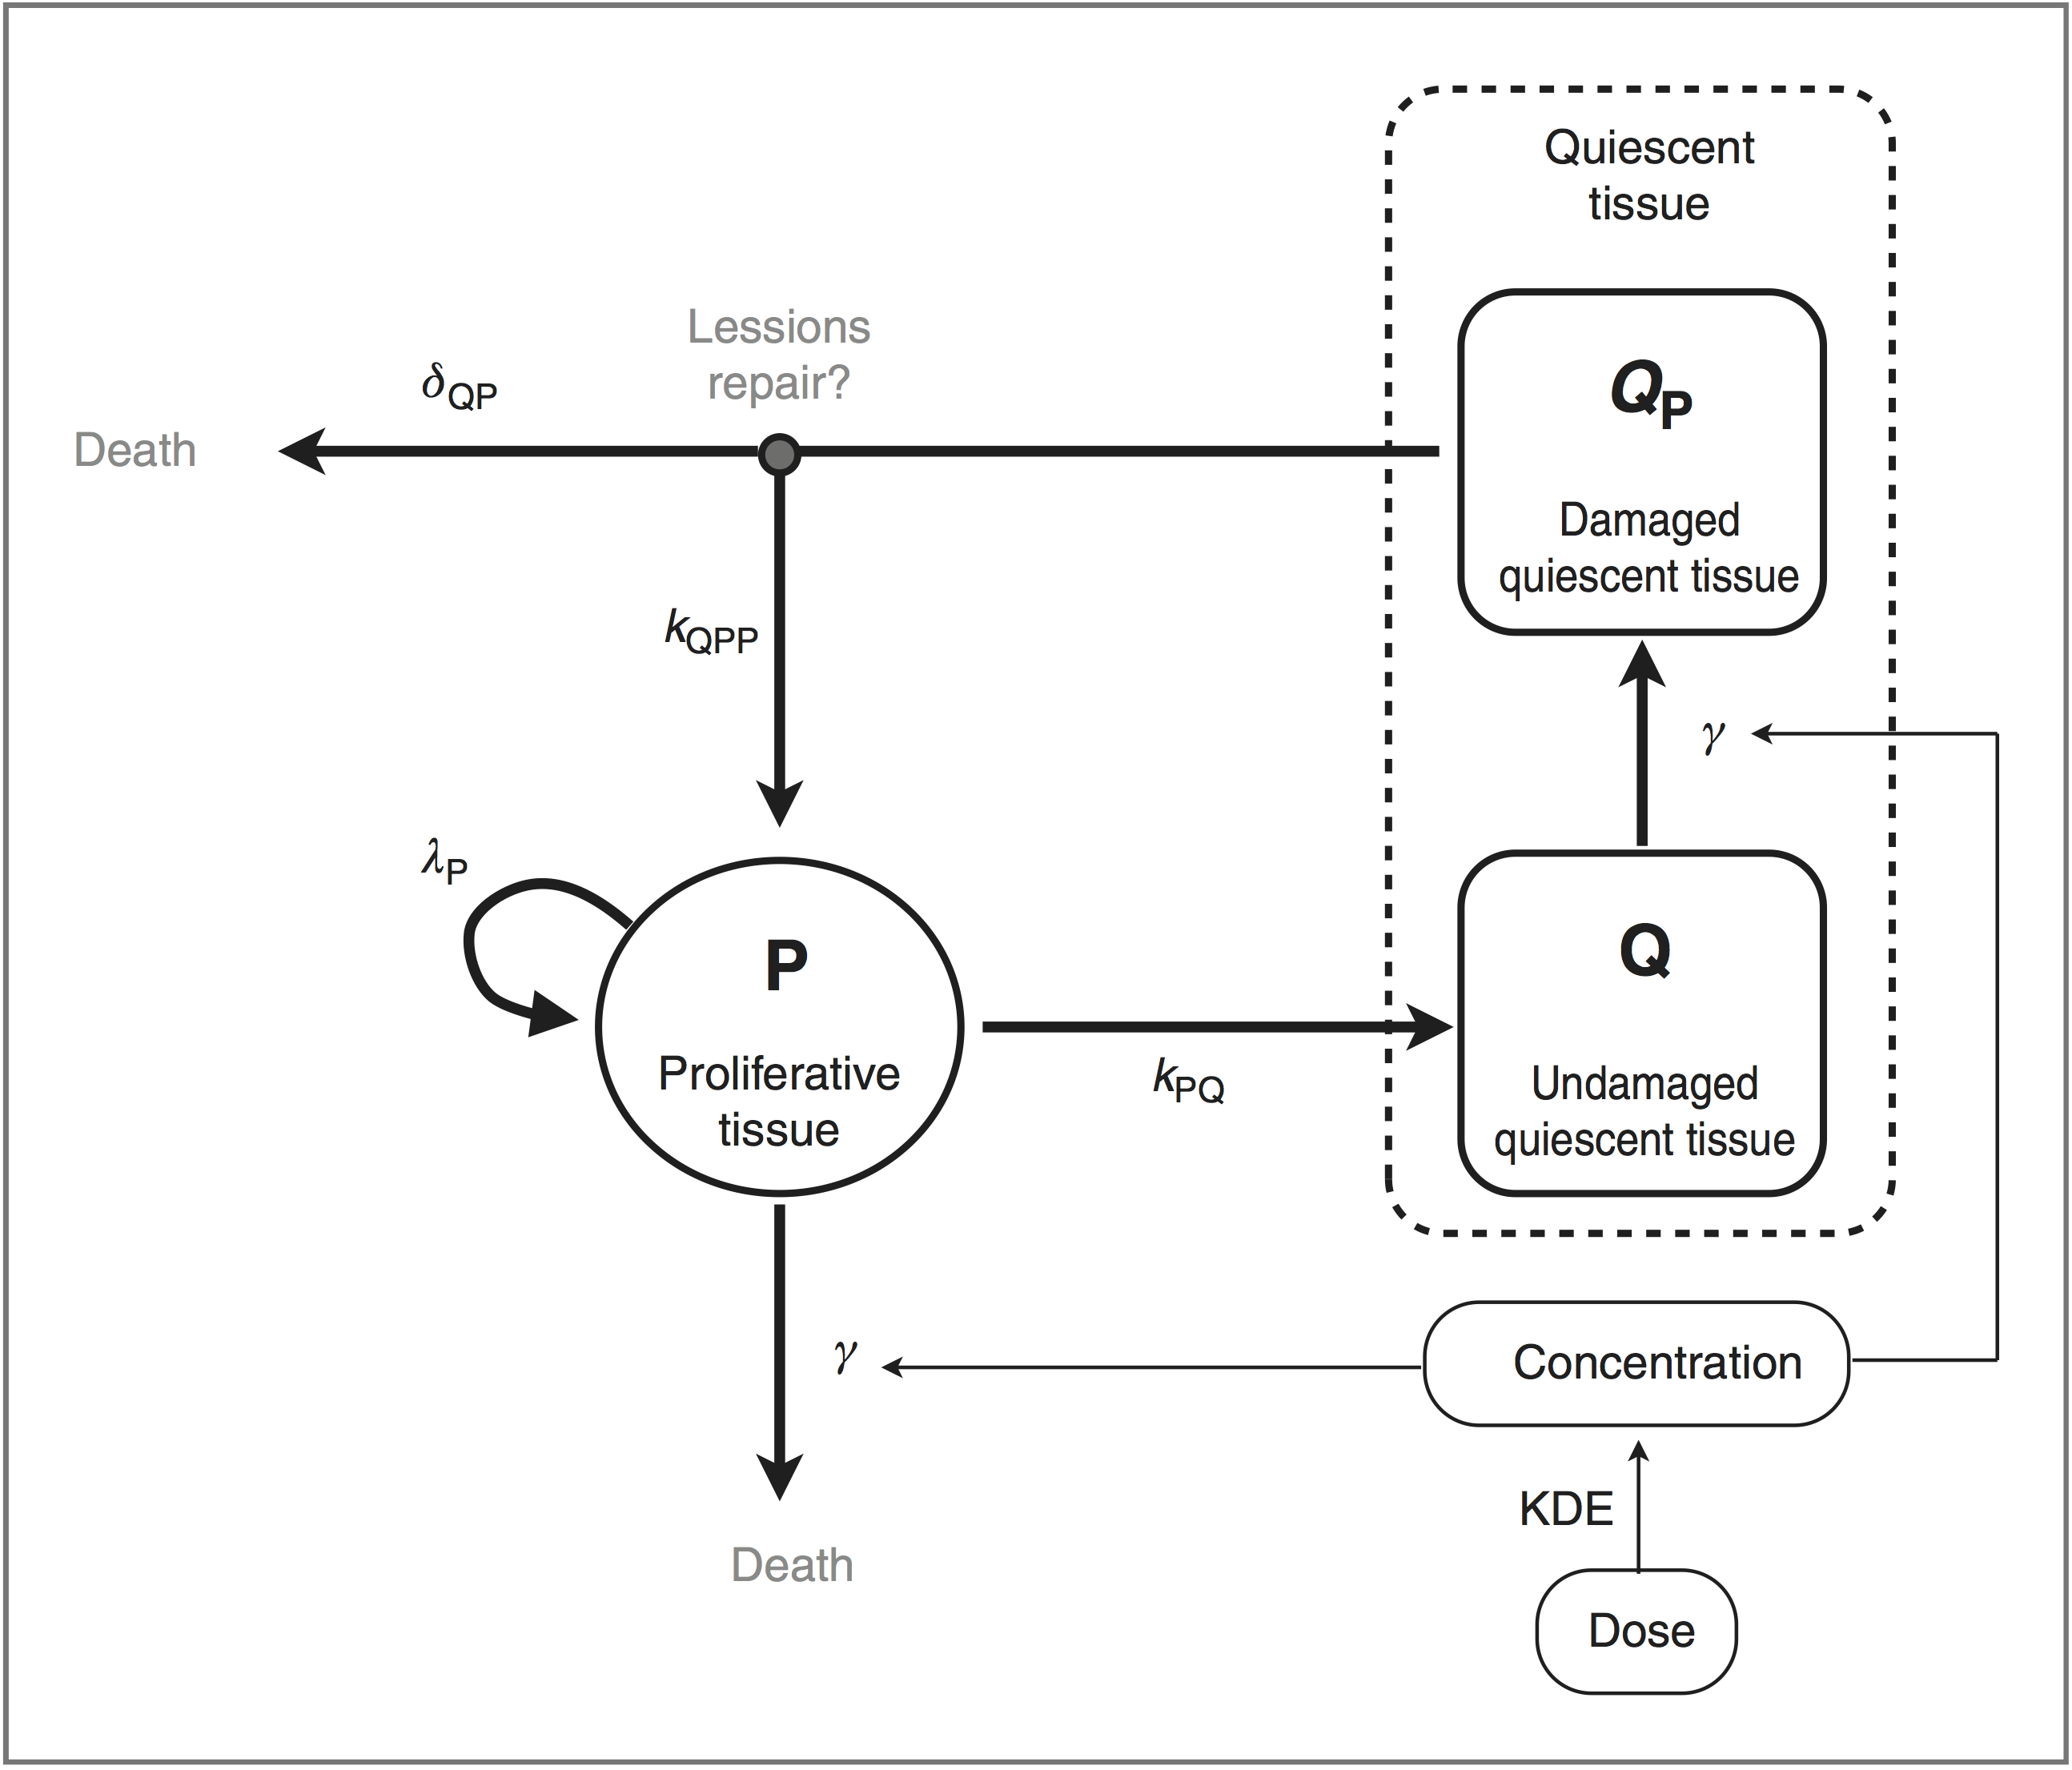
\includegraphics[angle=0,width=.8\textwidth]{modelo.png}
	\caption{\label{modelo}}
\end{figure}

Los autores aplicaron un modelo farmacocinético del PCV usando un enfoque cinético-farmacodinámico, en el cual se supone que la concentración del medicamento decae de acuerdo a una función exponencial. En el modelo, no se consideraron los tres medicamentos por separado, sino que se supuso que el tratamiento está representado como un todo, incluyendo los tres componentes quimoterapéuticos del tratamiento con PVC. SE modeló el número exacto de ciclos de tratamiento administrado al hacer 1 el valor de $C$ al inicio de cada ciclo. El modelo resultante es el siguiente:

\begin{align*}
\frac{dC}{dt}&=-KDE \,(C)\\
\frac{dP}{dt}&=\lambda_p \, P \left ( 1-\frac{P^*}{K}\right) + k_{Q_PP}\,Q_P-k_{PQ}\,P-\gamma_P\, C \, (KDE) \, P\\
\frac{dQ}{dt}&=k_{PQ}\,P-\gamma_Q \,C \, (KDE) \, Q\\
\frac{dQ_p}{dt}&=\gamma_Q \, C \, (KDE) \, Q - k_{Q_PP}Q_P-\delta_{QP}\,Q_P\\
P^*&=P+Q+Q_p
\end{align*} 

El parámetro $KDE$ es la tasa de decaimiento constante de la concentración de PVC en plasma, denotada C. $\lambda_p$ es la tasa de crecimiento constante usada en el modelo logístico para la expansión del tejido proliferativo. Se asume que la concentración del medicamento C induce daños en el ADN tanto en el tejido proliferativo como en el tejido latente por medio de funciones lineales; el daño se representa respectivamente por $\gamma_P$ y $\gamma_Q$. También se supone que $\gamma_P=\gamma_Q=\gamma$, lo cual se puede justificar por el hecho de que la acción básica del tratamiento puede no depender del ciclo celular del que se hable. 

Los autores dicen haber probado varias expresiones para el crecimiento del tejido proliferativo y eligieron la ecuación logística con un tamaño máximo del tumor de 100 mm porque es la que les dio mejores resultados y porque ese tamaño es consistente con los pacientes con LGG. El parámetro $k_{Q_PP}$ es la tasa constante de transferencia del tejido latente dañado al tejido proliferativo y $\delta_{QP}$ representa el tasa constante de eliminación del tejido latente. 

Los parámetros del modelo se estimaron al ajustar la solución del modelo $P+Q+Q_P$ a los valores reales a la MTD. El conjunto de parámetros resultante por estimar fue $\{ \lambda_P,k_{PQ},k_{Q_PP},\delta_{Q_P},\gamma, KDE\}$ con dos condiciones adicionales $P(t=0)=P_0$ y $Q(t=0)=Q_0$, donde el tiempo $t=0$ corresponde a los primeros datos disponibles. Se asumió también que $Q_{P_0}=Q_P(t=0)=0$ en la ausencia de tratamiento. 

Los parámetros individuales que corresponden a los ocho parámetros de la población se asume que se distribuyen de modo lognormal entre los individuos. La variabilidad de KDE se tomó como fija y todos los demás parámetros se estimaron con su variabilidad interindividual.

En el modelo se considera que $\lambda_p$ y $k_{PQ}$ son parámetros específicos del tumor, ya que en la ausencia de tratamiento, el sistema se reduce a otro en l cual solo estoys dos parámetros regulan el crecimiento del tumor. Los parámetros restantes, $(k_{Q_PP},\delta_{Q_P},\gamma, KDE)$ se pueden considerar como parámetros relativos al tratamiento. Lo cierto es que todos los parámetros juntos regulan las características de la respuesta del tumor al tratamiento, especialmente el encogimiento del tumor y la duración de la respuesta.

\subsection{Simplificación del modelo}

El modelo se simplificó para ver las diferencias que existían con el modelo original de Ribba et al. La simplificación consistió en considerar al tejido latente sin hacer la diferencia entre tejido dañado y no dañado. El esquema del modelo simplificado se muestra en la figura (\ref{modelosimple}). El sistema de ecuaciones diferenciales resultante es el siguiente:

\begin{figure}[h]
	\centering
	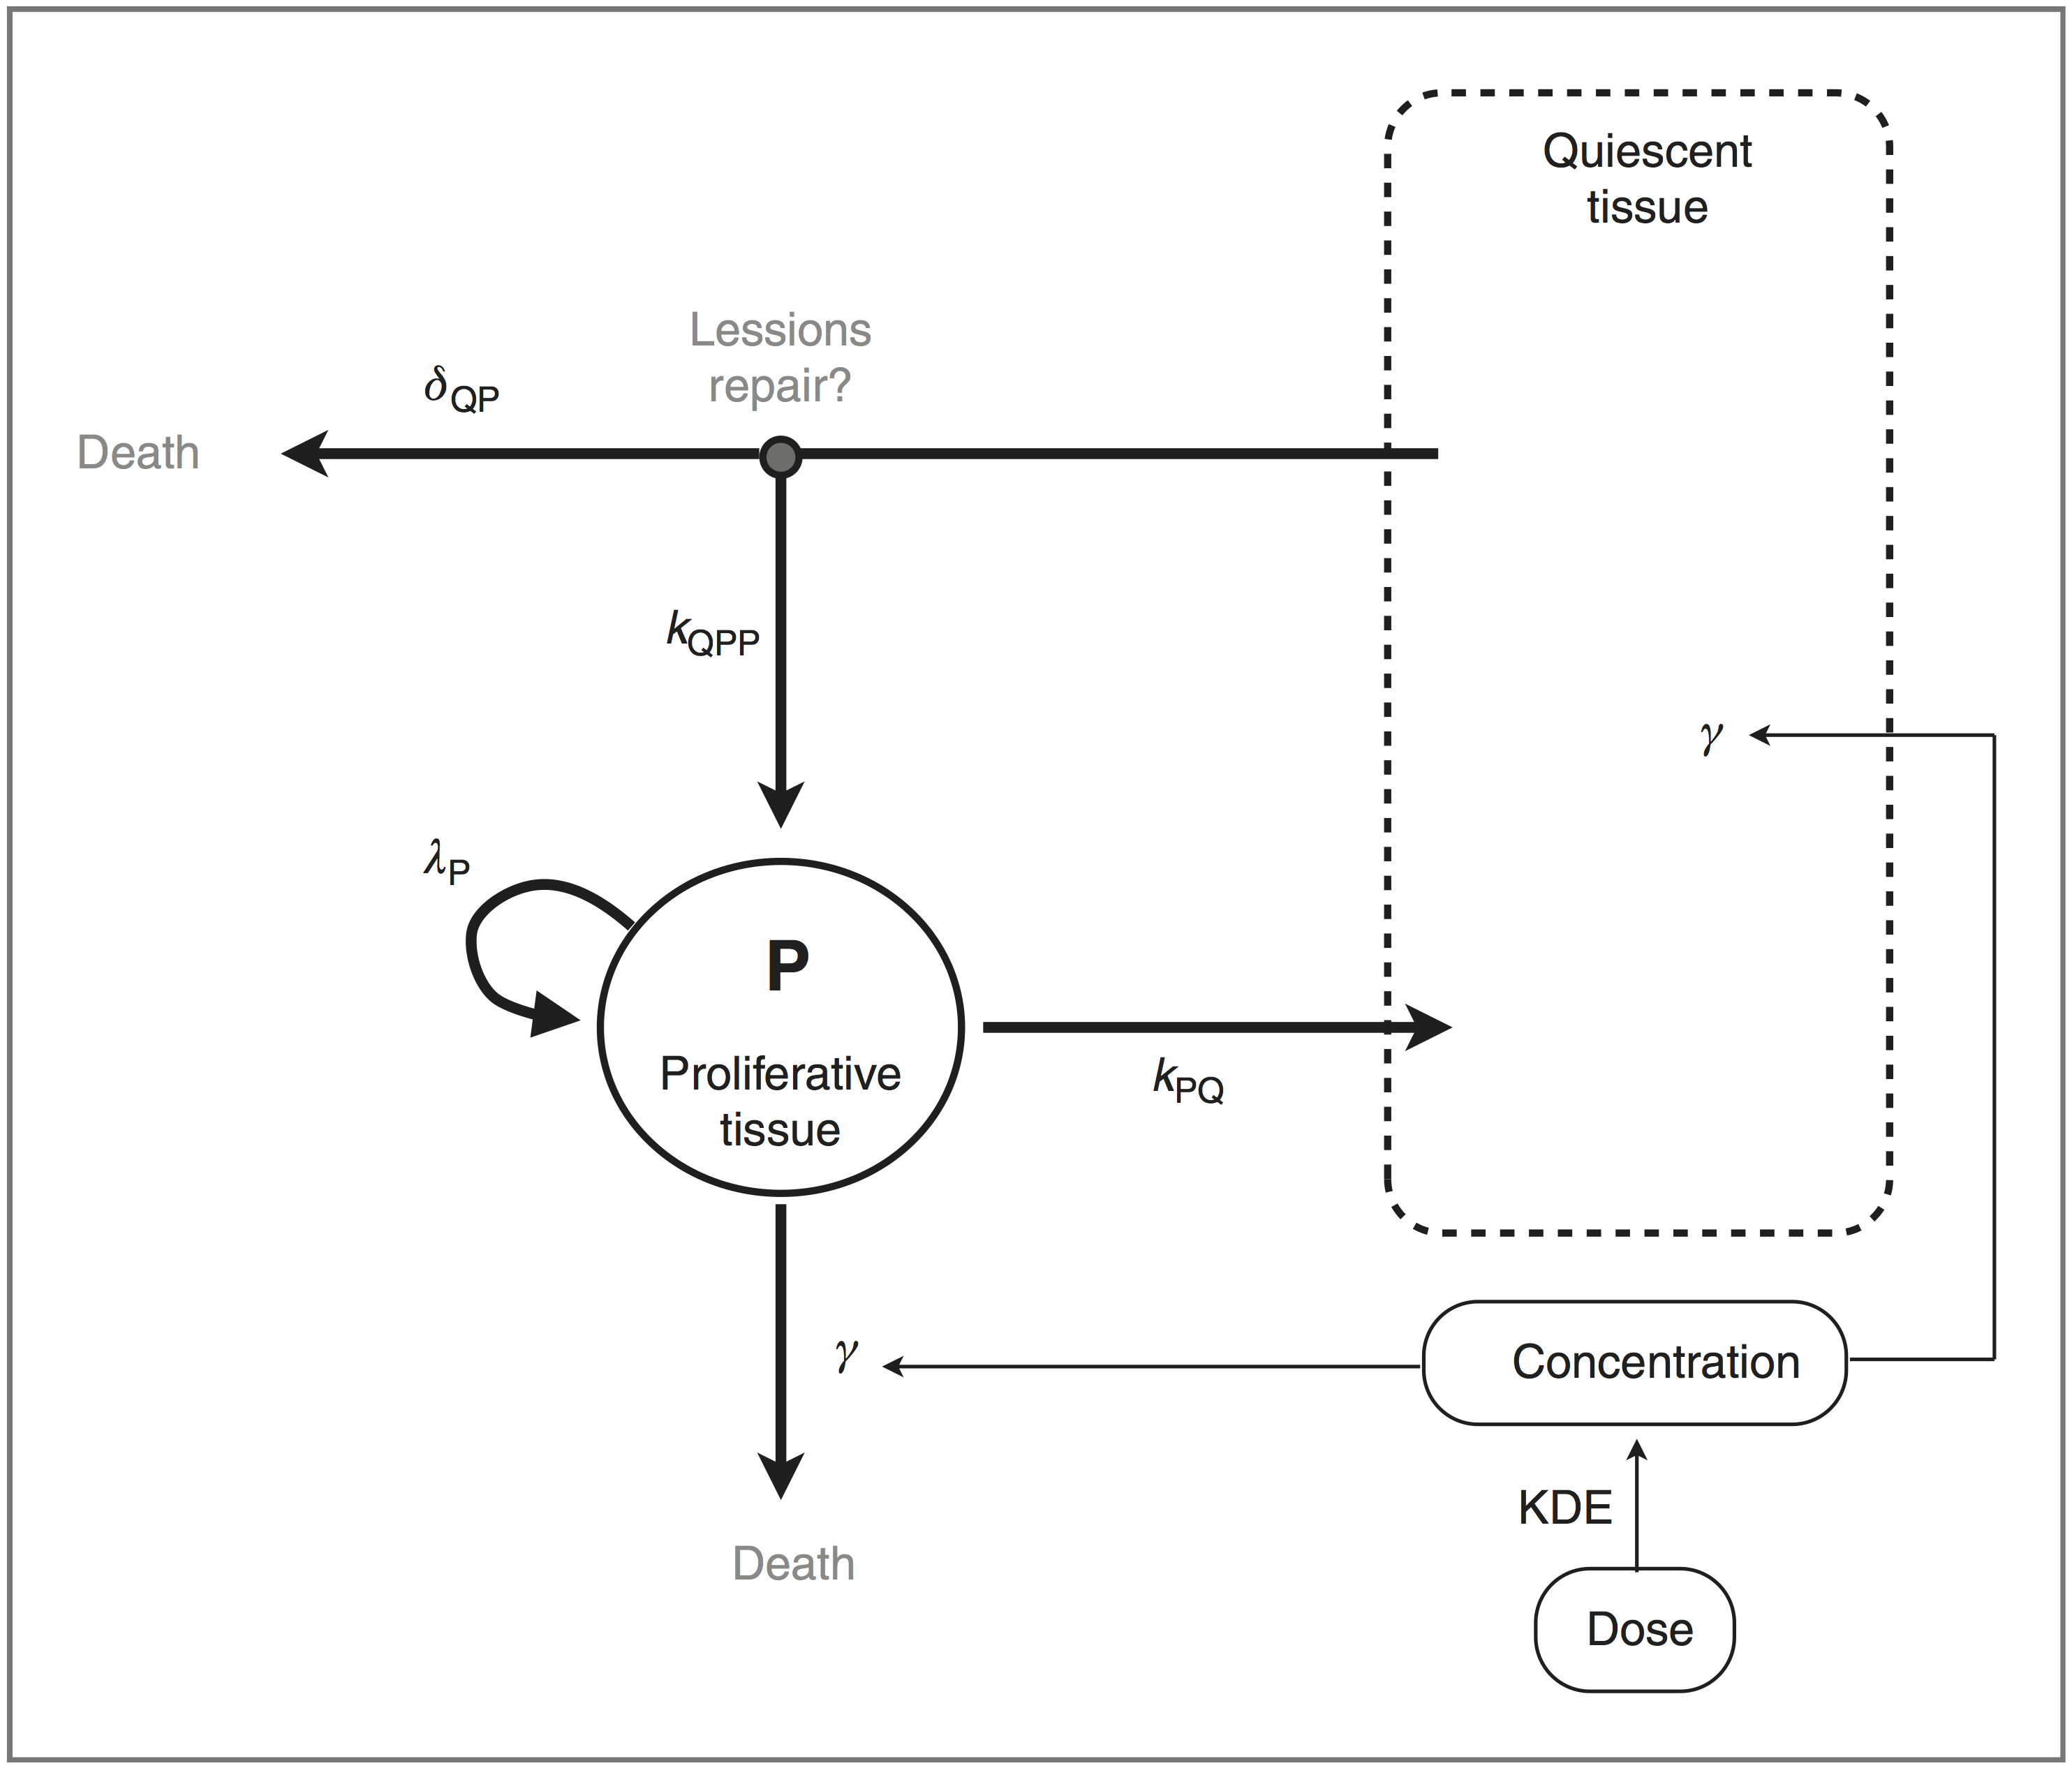
\includegraphics[angle=0,width=.8\textwidth]{modelosimple.png}
	\caption{\label{modelosimple}}
\end{figure}

\begin{align*}
\frac{dC}{dt}&=-KDE \,(C)\\
\frac{dP}{dt}&=\lambda_p \, P \left ( 1-\frac{P^*}{K}\right) + k_{Q_PP}\,Q_P-k_{PQ}\,P-\gamma_P\, C \, (KDE) \, P\\
\frac{dQ}{dt}&=k_{PQ}\,P- k_{QP}Q-\delta_{QP}\,Q\\
P^*&=P+Q+Q_p
\end{align*} 

\section{Resultados}

Los resultados obtenidos por Monolix, eligiendo la configuración del software por defecto salvo $k_1$=400 y $k_2=300$ (parámetros del algoritmo de esperanza-maximización por aproximación estocástica) y con un modelo de error proporcional son los siguientes:

\subsection{Modelo original}

\begin{verbatim}
******************************************************************
*      tumor1aproportional.mlxtran
*      August 02, 2016 at 16:50:48
*      Monolix version: 4.4.0
******************************************************************

Estimation of the population parameters

               parameter     s.e. (s.a.)   r.s.e.(%) 
kde_pop      :    0.123         0.029          23    
kPQ_pop      :   0.0283         0.013          46    
kQpP_pop     :  0.00462        0.0023          49    
lambda_pop   :    0.115         0.026          22    
gamma_pop    :    0.804          0.28          35    
delta_pop    :  0.00387        0.0013          34    
P0_pop       :        9           3.3          36    
Q0_pop       :     38.4           4.2          11    

omega_kde    :    0.334          0.18          53    
omega_kPQ    :    0.878          0.49          56    
omega_kQpP   :    0.529          0.55         104    
omega_lambda :    0.659          0.22          33    
omega_gamma  :    0.721          0.23          32    
omega_delta  :    0.576          0.39          67    
omega_P0     :    0.859          0.21          24    
omega_Q0     :    0.272         0.072          26    

b            :   0.0499         0.003           6    

______________________________________________
correlation matrix of the estimates(Stochastic Approximation)

kde_pop         1                      
kPQ_pop     -0.15       1                   
kQpP_pop    -0.46    0.62       1                
lambda_pop  -0.23    0.49    0.36       1             
gamma_pop   -0.41    0.44    0.48     0.5       1          
delta_pop    0.55   -0.02   -0.25   -0.03    -0.4       1       
P0_pop      -0.15    0.14    0.12   -0.16   -0.28   -0.13       1    
Q0_pop       0.19   -0.21   -0.17    0.08    0.22    0.13   -0.67       1 

Eigenvalues (min, max, max/min): 0.24  2.9  12

omega_kde         1                         
omega_kPQ       0.1       1                      
omega_kQpP    -0.37   -0.25       1                   
omega_lambda   0.26    0.47   -0.56       1                
omega_gamma   -0.25   -0.31    0.61   -0.49       1             
omega_delta    0.26    0.35    -0.6    0.47   -0.56       1          
omega_P0       0.11   -0.03   -0.29   -0.04   -0.21    0.31       1       
omega_Q0      -0.09   -0.05    0.35   -0.03    0.28   -0.35   -0.53       1    
b             -0.26   -0.22    0.15   -0.21    0.11   -0.18   -0.06    0.04       1 

Eigenvalues (min, max, max/min): 0.3  3.4  11


Population parameters and Fisher Information Matrix estimation...

Elapsed time is 228 seconds. 
CPU time is 595 seconds. 
______________________________________________________________

Log-likelihood Estimation by Importance Sampling
Sampling distribution for the random effects: t with 5 d.f

-2 x log-likelihood:                   1515.31 (2.1)
Akaike Information Criteria   (AIC):   1549.31 (2.1)
Bayesian Information Criteria (BIC):   1567.07 (2.1)

Elapsed time is 62.3 seconds. 
CPU time is 223 seconds. 
______________________________________________________________
\end{verbatim}

\begin{figure}[h]
	\centering
	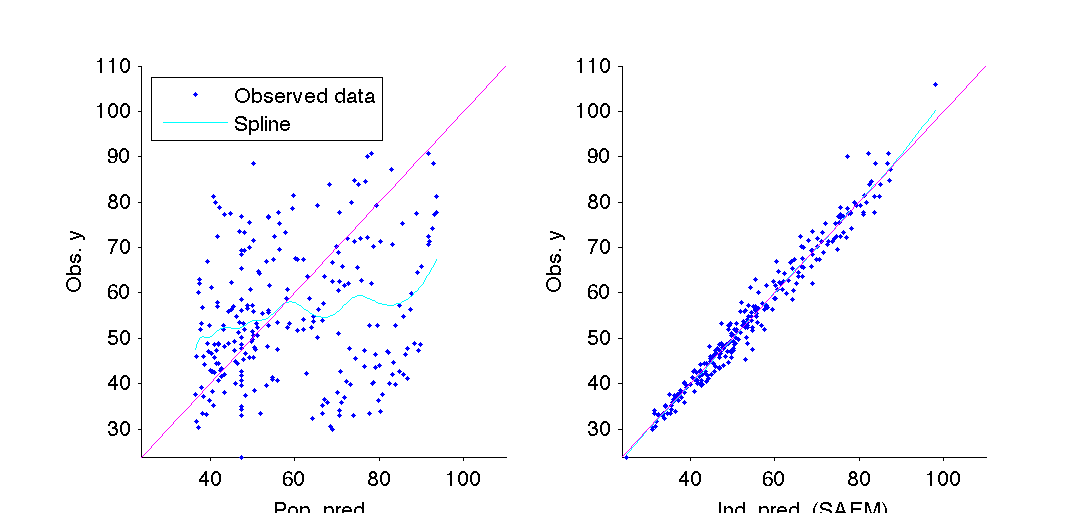
\includegraphics[angle=0,width=.8\textwidth]{predVsObs.png}
	\caption{\label{PvsO}Predicciones contra observaciones del modelo original.}
\end{figure}

\subsection{Modelo simplificado}
\begin{verbatim}
******************************************************************
*      tumor2proportional.mlxtran
*      August 02, 2016 at 16:19:59
*      Monolix version: 4.4.0
******************************************************************

Estimation of the population parameters

               parameter     s.e. (s.a.)   r.s.e.(%) 
kde_pop      :    0.115         0.031          27    
kPQ_pop      :   0.0528         0.013          24    
kQP_pop      :  0.00349        0.0018          51    
lambda_pop   :    0.136         0.022          16    
gamma_pop    :     0.72          0.36          50    
delta_pop    :  0.00293        0.0025          87    
P0_pop       :     7.89           3.7          47    
Q0_pop       :     38.2           3.7          10    

omega_kde    :    0.325          0.25          77    
omega_kPQ    :    0.436          0.26          60    
omega_kQP    :    0.929           0.4          43    
omega_lambda :    0.505          0.15          29    
omega_gamma  :    0.706           0.4          57    
omega_delta  :    0.995           0.7          70    
omega_P0     :     1.19          0.36          30    
omega_Q0     :    0.264         0.058          22    

b            :   0.0506        0.0029           6    

______________________________________________
correlation matrix of the estimates(Stochastic Approximation)

kde_pop         1                      
kPQ_pop     -0.31       1                   
kQP_pop     -0.62    0.53       1                
lambda_pop  -0.03    0.37    0.01       1             
gamma_pop   -0.68    0.47    0.52    0.28       1          
delta_pop    0.74   -0.39   -0.56   -0.12   -0.86       1       
P0_pop       0.51   -0.24   -0.33   -0.22   -0.67    0.64       1    
Q0_pop      -0.37    0.07    0.24    0.12    0.48   -0.46   -0.56       1 

Eigenvalues (min, max, max/min): 0.12  4.1  33

omega_kde         1                         
omega_kPQ     -0.48       1                      
omega_kQP     -0.17    0.17       1                   
omega_lambda   0.24   -0.27   -0.37       1                
omega_gamma   -0.65    0.51     0.1   -0.25       1             
omega_delta    0.66    -0.5   -0.29    0.31    -0.7       1          
omega_P0       0.51   -0.54   -0.12    0.18   -0.57    0.55       1       
omega_Q0       0.05   -0.06   -0.08     0.1   -0.03    0.06   -0.03       1    
b             -0.15    0.02       0   -0.11     0.1   -0.13   -0.08   -0.06       1 

Eigenvalues (min, max, max/min): 0.27  3.5  13


Population parameters and Fisher Information Matrix estimation...

Elapsed time is 229 seconds. 
CPU time is 581 seconds. 
______________________________________________________________

Log-likelihood Estimation by Importance Sampling
Sampling distribution for the random effects: t with 5 d.f

-2 x log-likelihood:                   1521.93 (2.6)
Akaike Information Criteria   (AIC):   1555.93 (2.6)
Bayesian Information Criteria (BIC):   1573.68 (2.6)

Elapsed time is 63 seconds. 
CPU time is 215 seconds. 
______________________________________________________________

\end{verbatim}

\begin{figure}[h]
	\centering
	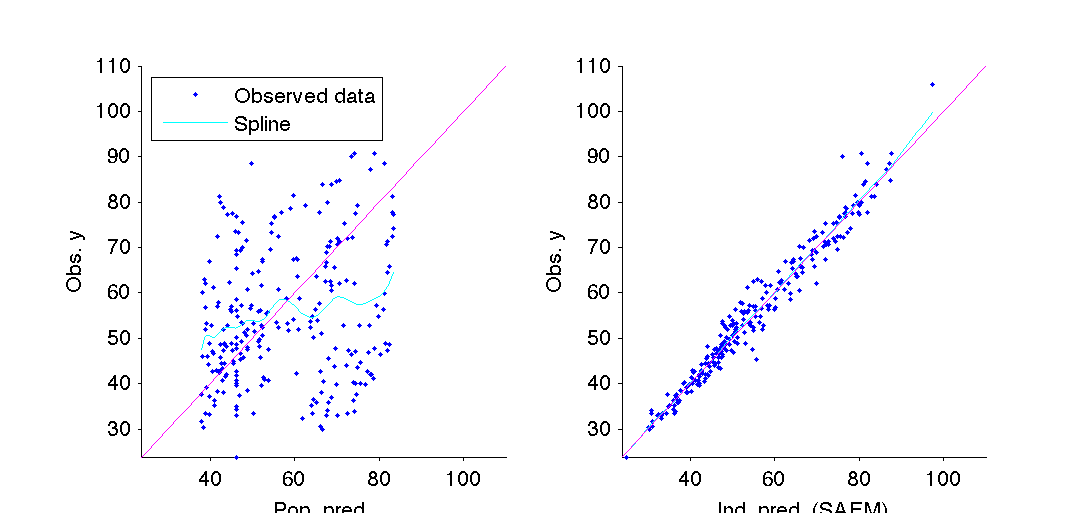
\includegraphics[angle=0,width=.8\textwidth]{predVsObs2.png}
	\caption{\label{PvsO2}Predicciones contra observaciones del modelo simplificado.}
\end{figure}

\section{Conclusiones}

Como puede verse en las gráficas (\ref{PvsO}) y (\ref{PvsO2}), ambos modelos aproximan bien a los datos. Lo que es más, observando el criterio de información de Bayes, no existe una diferencia significativa entre el modelo original y el simplificado. Lo cierto es que el tiempo de ejecución computacional es de más del doble para el modelo original que para el simplificado. Basándose en estas observaciones, el modelo simplificado parece suficiente para describir el cambio del tamaño del tumor en el tiempo.

\end{document}
